\documentclass[a4paper, 11pt]{tufte-handout}
\usepackage[margin=0.1in]{geometry}
\geometry{
    textwidth=4.5in,
}
\usepackage{framed}
\usepackage[brazil]{babel}
\usepackage{graphicx}
\usepackage{xcolor}
\usepackage{verbatim}
\usepackage{blindtext}
\usepackage{xcolor}
% The following package makes prettier tables.  We're all about the bling!
\usepackage{booktabs}
% The units package provides nice, non-stacked fractions and better spacing
% for units.
\usepackage{units}
% \usepackage{mdframed}
\usepackage{indentfirst}
\usepackage{hyperref}
% \usepackage{txfonts}
\usepackage{amsmath}
\usepackage{titling}
\usepackage{titlesec}

\definecolor{LightGray}{gray}{0.97}
\usepackage{minted}

\usepackage{xcolor} % to access the named colour LightGray

\setminted[fortran]{  framesep=2mm,
  baselinestretch=1.2,
  bgcolor=LightGray,
  fontsize=\footnotesize,
  linenos}

\titleformat{\section}{\normalfont\Large\bfseries}{\thesection}{1em}{}[\titlerule] 
\titleformat{\subsection}{\normalfont\large\bfseries}{\thesubsection}{1em}{} 
% \renewcommand\thesubsection{\Alph{subsection}}
\graphicspath{ {./graficos/} }

\hypersetup{
  pdfauthor={Jefter Santiago},
  pdftitle={Projeto 2 - Equações de Onda I},
%  pdfkeywords={},
%  pdfsubject={Anotações métodos matemáticos aplicados à física},
  pdfcreator={Jefter Santiago}, 
  pdflang={Portuguese},
  colorlinks=true,    % Color links instead of boxes
  linkcolor=blue,     % Color of internal links
  citecolor=green,    % Color of citation links
  urlcolor=blue,      % Color of URLs
}
\begin{document}
\begin{fullwidth}
\noindent
\large\textbf{Autor:} Jefter Santiago \hfill \textbf{Projeto 2: {\color{blue}\emph{Equações de ondas I}}}   \\
\#USP: 12559016 \\
\normalsize Curso: Física Estatística Computacional \\
Prof. F. C. Alcaraz \hfill Data de entrega: 06/04/2024\\
\noindent\rule{7in}{2.8pt}
\end{fullwidth}


\section{Discretização da Equação de Onda}
Nesse trabalhamo buscamos estudar a equação do onda em 1D, para isso partimos da equação
(\ref{eq:eq_onda}) e fazemos a sua discretização. Escolhemos utilizar a discretização para derivadas
simétricas, e portanto obtemos a forma da equação de ondas com a qual trabalharemos (\ref{eq:ondas_discreta})
\begin{equation}
  \frac{\partial^2 \mathcal{Y}}{\partial t^2} = c^2  \frac{\partial^2 \mathcal{Y}}{\partial x^2}
  \label{eq:eq_onda}
\end{equation}

Partindo das derivadas segundas, com \( x = i \Delta x \) e \( t = n \Delta t \) para \( i, n = 1, 2, ... \)  temos
\[  \frac{\mathcal{Y}(i, n+1) + \mathcal{Y}(i,n-1) - 2 \mathcal{Y}(i,n)}{(\Delta t)^2} = c^2 \frac{\mathcal{Y}(i+1,n) + \mathcal{Y}(i-1,n) -
    2\mathcal{Y}(i,n)}{(\Delta x)^2} \]

\[ \mathcal{Y}(i, n+1) + \mathcal{Y}(i,n-1) - 2 \mathcal{Y}(i,n) = \frac{c^2 (\Delta t)^2}{(\Delta x)^2} \left[ \mathcal{Y}(i+1, n) + \mathcal{Y}(i-1,n) - 2\mathcal{Y}(i,n) \right]  \]

fazendo  \( r \equiv  c \Delta t/\Delta x\) podemos escrever as iterações no tempo para cada posição da propagação
na equação abaixo

\begin{equation}
  \mathcal{Y}(i, n+1) = 2 \left( 1 - r^2 \right) \mathcal{Y}(i, n) + r^2 \left( \mathcal{Y}(i+1,n) + \mathcal{Y}(i-1,n) \right) - \mathcal{Y}(i,n-1)
  \label{eq:ondas_discreta}
\end{equation}


Fica claro pela equação (\ref{eq:ondas_discreta}) que para nossa simulação podemos trabalhar com 
vetores que descrevem o estado de uma posição em cada posição, ``anterior'', ``atual'' e
``posterior''. No código das simulações foi implementado uma matrix ``grid'' que computa esses
estados de acordo com a iteração.  

Para finalizar a descrição do problema de propagação de ondas precisamos das condições de
contorno. Nesse projeto inicial foram feitas simulações em condições para propagação ideal de ondas
presas em uma caixa, ou seja, nas extremidades do nosso espaço vale que $\mathcal{Y}(0) = \mathcal{Y}(L) = 0$, para um
comprimento $L$ qualquer e $d \mathcal{Y}(x, t = 0)/ dt = 0$. 

\subsection{Estabilidade numérica}
\label{sec:estabilidade}
A escolha dos menores \( \Delta x \) e \( \Delta t \) em geral levam a execuções mais estáveis. Porém, quando
trabalhamos com dois passos diferentes surgem algumas possíveis instabilidades. Buscando simplificar
essas análises escrevemos o fator $r$

\begin{equation}
  r = \frac{\Delta t}{\Delta x} c
  \label{eq:fator_r}
\end{equation}

a partir dessa relação podemos tirar algumas conclusões: \( \Delta x \) e \( \Delta t \) devem variar juntos,
pois se mantermos um deles fixo e variando o outro obtemos uma divergência, por exemplo se \( \Delta x \)
são valores cada vez menores para um \( \Delta t \) fixo e o caso mais estável que podemos obter é no
qual \( r = 1  \).

No projeto iniciamos as simulações no caso mais estável de uma onda ideal com \( r = 1 \) e depois
as situações em que as instabilidades numéricas surgem. Nesses casos foi necessário trabalhar com
menos interações já que os valores de $Y$ divergem muito rapidamente. Então basta algumas iterações
para demonstrarmos esta instabilidade.


\subsection{Erro associado à simulação}
\label{sec:erro}

Pela relação (\ref{eq:ondas_discreta}), temos um erro associado à \( x \) que buscamos
minimizar. No trabalho estamos usando números de precisão de 12 e portanto, o termo de
erro da derivada segunda é a ordem que ``escondemos'' na equação de ondas discretizada

\begin{equation}
  \mathcal{E}(\Delta x) =  \Delta x^2 + \frac{10^{-12}}{(\Delta x)^2}
\end{equation}

o ponto de mínimo desse erro é em torno de \( \Delta x = 10^{-3} \), portanto esse é o nosso mínimo.

Partindo desse valor para \( \Delta x\) fixo trabalhamos variando os outros e observando qual a
influência deles na instabilidade do algoritmo.

\section{Simulações de ondas ideais}


Como foi discutido anteriormente (\ref{sec:erro}) o $\Delta x$ escolhido
foi fixado para todas simulações. Além disso a velocidade de nossas ondas também é mantida constante
igual à \( c = 300\) (m/s). Com isso podemos variar os paramêtros de \( r \) e \( \Delta t \). 

Foi escolhido um periodo total de \( t = 0,01\)(s)  de forma que, para uma onda à velocidade da luz
dentro de uma caixa de \( 1\)(m) hajam 3 reflexões.


Foram utilizadas as mesmas rotinas para implementação da simulação com uma única mudança, as
condições iniciais, já que as condições de contorno, isto é, a corda presa nas extremidades, é
válida para simulação das ondas na corda de um violão. Para a simulação de ondas Gaussianas usamos o
modelo de condição inicial dado por 

\begin{equation}
    \mathcal{Y}(x, 0) = \mathcal{Y}_0 (x) = \exp{\left[- \frac{(x-x_0)^2}{\sigma^2}\right]}, x_0 = L/3, \sigma = L/30 \\
  \label{eq:y_0}
\end{equation}
\( d \mathcal{Y} / d t |_{t = 0} = 0 \)
onde no código foi denotado por  \verb|Y0(x,s)|.


Segue abaixo abaixo a estrutura central do programa de simulação de ondas:

\begin{minted}{fortran}[!]
!     Simulação para ondas ideias
      implicit real*8(a-h, o-y)
      dimension grid(1000, 3)
      ! L 
      s = 1.0d0
      c = 300.0d0
      r = 1.0d0
      nx = 1000
      dx = s / (nx*1.d0)
      dt = r * dx / c
      t = 0.01
      nt = floor(t/dt)
      open(unit = 1, file = "saida-tarefa1-a.dat")
      grid(:, 3) = 0.e0
!     aplica as condicoes iniciais ao grid
!     t = 0
      do i = 1, nx
         grid(i, 2) = Y0(i*dx, s)
      end do
!     
      grid(:,1) = grid(:, 2)
      call write_to_file(grid, nx)
!     t = 1
      grid(:, 2) = grid(:, 1)
!     simulação
      do n = 3, nt
         call drive_pulse(grid, nx, r)
         call write_to_file(grid, nx)
      end do
      close(1)
      end

      subroutine write_to_file(grid, nx)
      implicit real*8(a-h, o-y)
      dimension grid(1000, 3)
      write(1, '(3000F16.8)') (grid(i, 2), i=1, nx)
      end subroutine write_to_file

      subroutine drive_pulse(grid, nx, r)
      implicit real*8(a-h, o-y)
      dimension grid(1000, 3)
!     y_next = 2(1-r^2)y_curr + r^2[y(t+1,n)+y(t-1,n)] - y_prev
      grid(1, 3) = grid(1, 2)
      grid(nx,3) = grid(nx, 2)

      y = 2.e0*(1.e0-r*r)

      do i = 2, nx-1
         grid(i,3)=y*grid(i,2)+r*r*(grid(i+1,2)+grid(i-1,2))-grid(i,1)
      end do
!     swap
      grid(:, 1) = grid(:, 2)
      grid(:, 2) = grid(:, 3)
      end subroutine drive_pulse
\end{minted}

Para o programa as simulações de ondas em uma corda temos a condição inicial dada por
(\ref{eq:y_0}), implementada por
\begin{minted}{fortran}[!]
      function Y0(x, s)
      implicit real*8(a-h, o-y)
      Y0 = exp(-((x-s/3)**2)/(s/30)**2)
      end
\end{minted}

condição aplicada à todo o grid na linhas linhas $17$ à $24$ do programa.


\subsection{Caso de \( r = 1 \) }

Como podemos ver na figura (\ref{fig:tarefa1-a}) a oscilação não apresenta nenhuma deformação, e
fazendo valores maiores de \( t \) e observando o comportamento da onda não surgem deformações para
\( r = 1 \). Para condição de contorno de bordas fixas é esperado que a onda seja espelhada nas
reflexões, e é o que observamos para os dois pacotes à esquerda e à direita. A primeira reflexão
acontece em torno da iteração 30  e a segunda na iteração 70.

Ocorrem interferências de forma construtiva, pois pelas condições impostas ambos se encontram sempre
do mesmo lado da reflexão e se somam formando a amplitude completa inicial.
A configuração inicial do sistema vai se repetir na iteração número $200$, isto é, no tempo
\( 200 \cdot \Delta t \). Como nosso \( \Delta t\) utilizado é dado pela (\ref{eq:fator_r}), então \( \Delta t = 1 \cdot
\Delta x / 300  \approx 3 \cdot 10^{-5} \) será a configuração inicial se repete em \( t = 0,06 \) (s). Esse
é o tempo necessário para cada um dos pacotes menores percorrerem \( 2 L\). Para um \( L \)
qualquer, temos então \( t = 2 L / c \) será o tempo em que a situação inicial surge novamente.


\begin{figure}[h!] 
    \centering
    \centering
    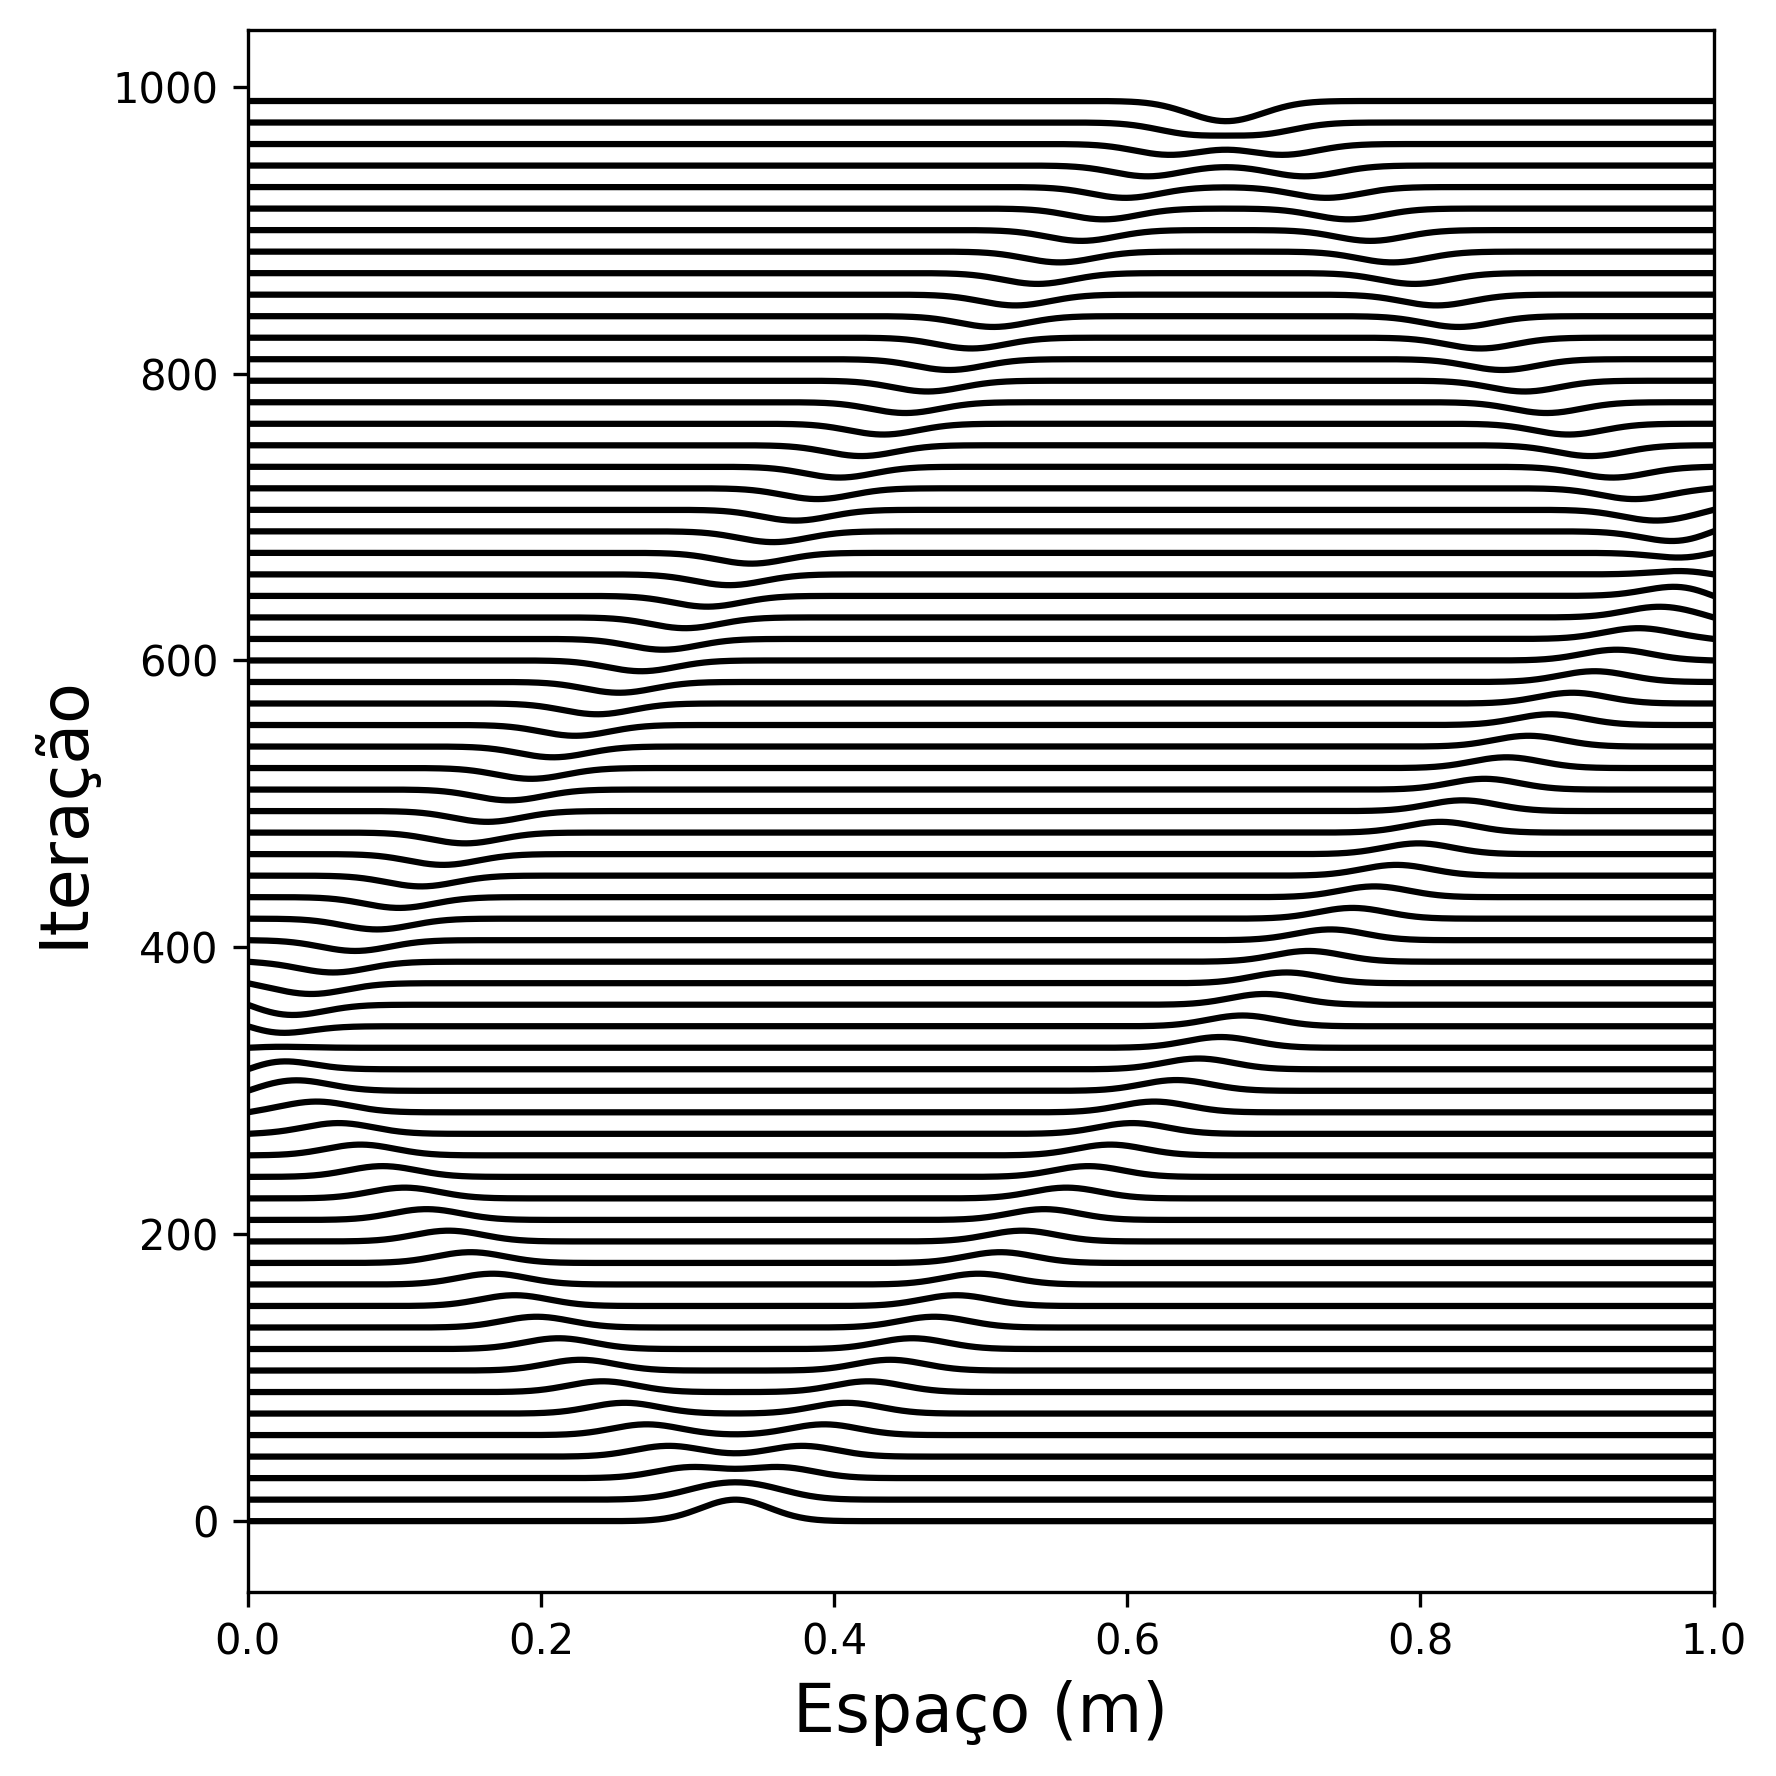
\includegraphics[width=0.5\linewidth]{graf-tarefa1-a}
    \caption{Evolução temporal da onda em $1000$ iterações. Apenas metade dessas iterações  estão nessa figura para melhor visualização das frentes de ondas.}
    \label{fig:tarefa1-a}
\end{figure}


\subsection{Caso de \( r = 2 \) }
\label{sec:caso_r_2}

Nesse caso podemos observar a instabilidade desse que surge para valores de \( r > 1  \).
A amplitude das ondas diverge muito rápido e na simulação bastaram pouquissímas iterações
para que visualizarmos o comportamento anômalo  da onda.

O algoritmo diverge para \( r > 1 \) pois, como foi discutido (\ref{sec:estabilidade}), a melhor
estabilidade que podemos ter é no caso em que \( r = 1 \). Podemos pensar em \( r = 2 \) como uma
diminuição do tamanho do passo \( \Delta x\) e como isso ocorre para um \( \Delta t \) fixo (já que $r$ mudou)
as pertubações que percorrem esse espaço à cada passo tem velocidade \( c \) em \( r = 1 \) passam a
ter velocidade menor que \( c \) e portanto cada iteração vai acumular valores cada vez maiores
vindos dessas pertubações que se somam, fazendo a amplitude divergir rapidamente.


\begin{figure}[h!] 
    \centering
    \caption{Divergência da equação da solução para \( r = 2 \).
    }
    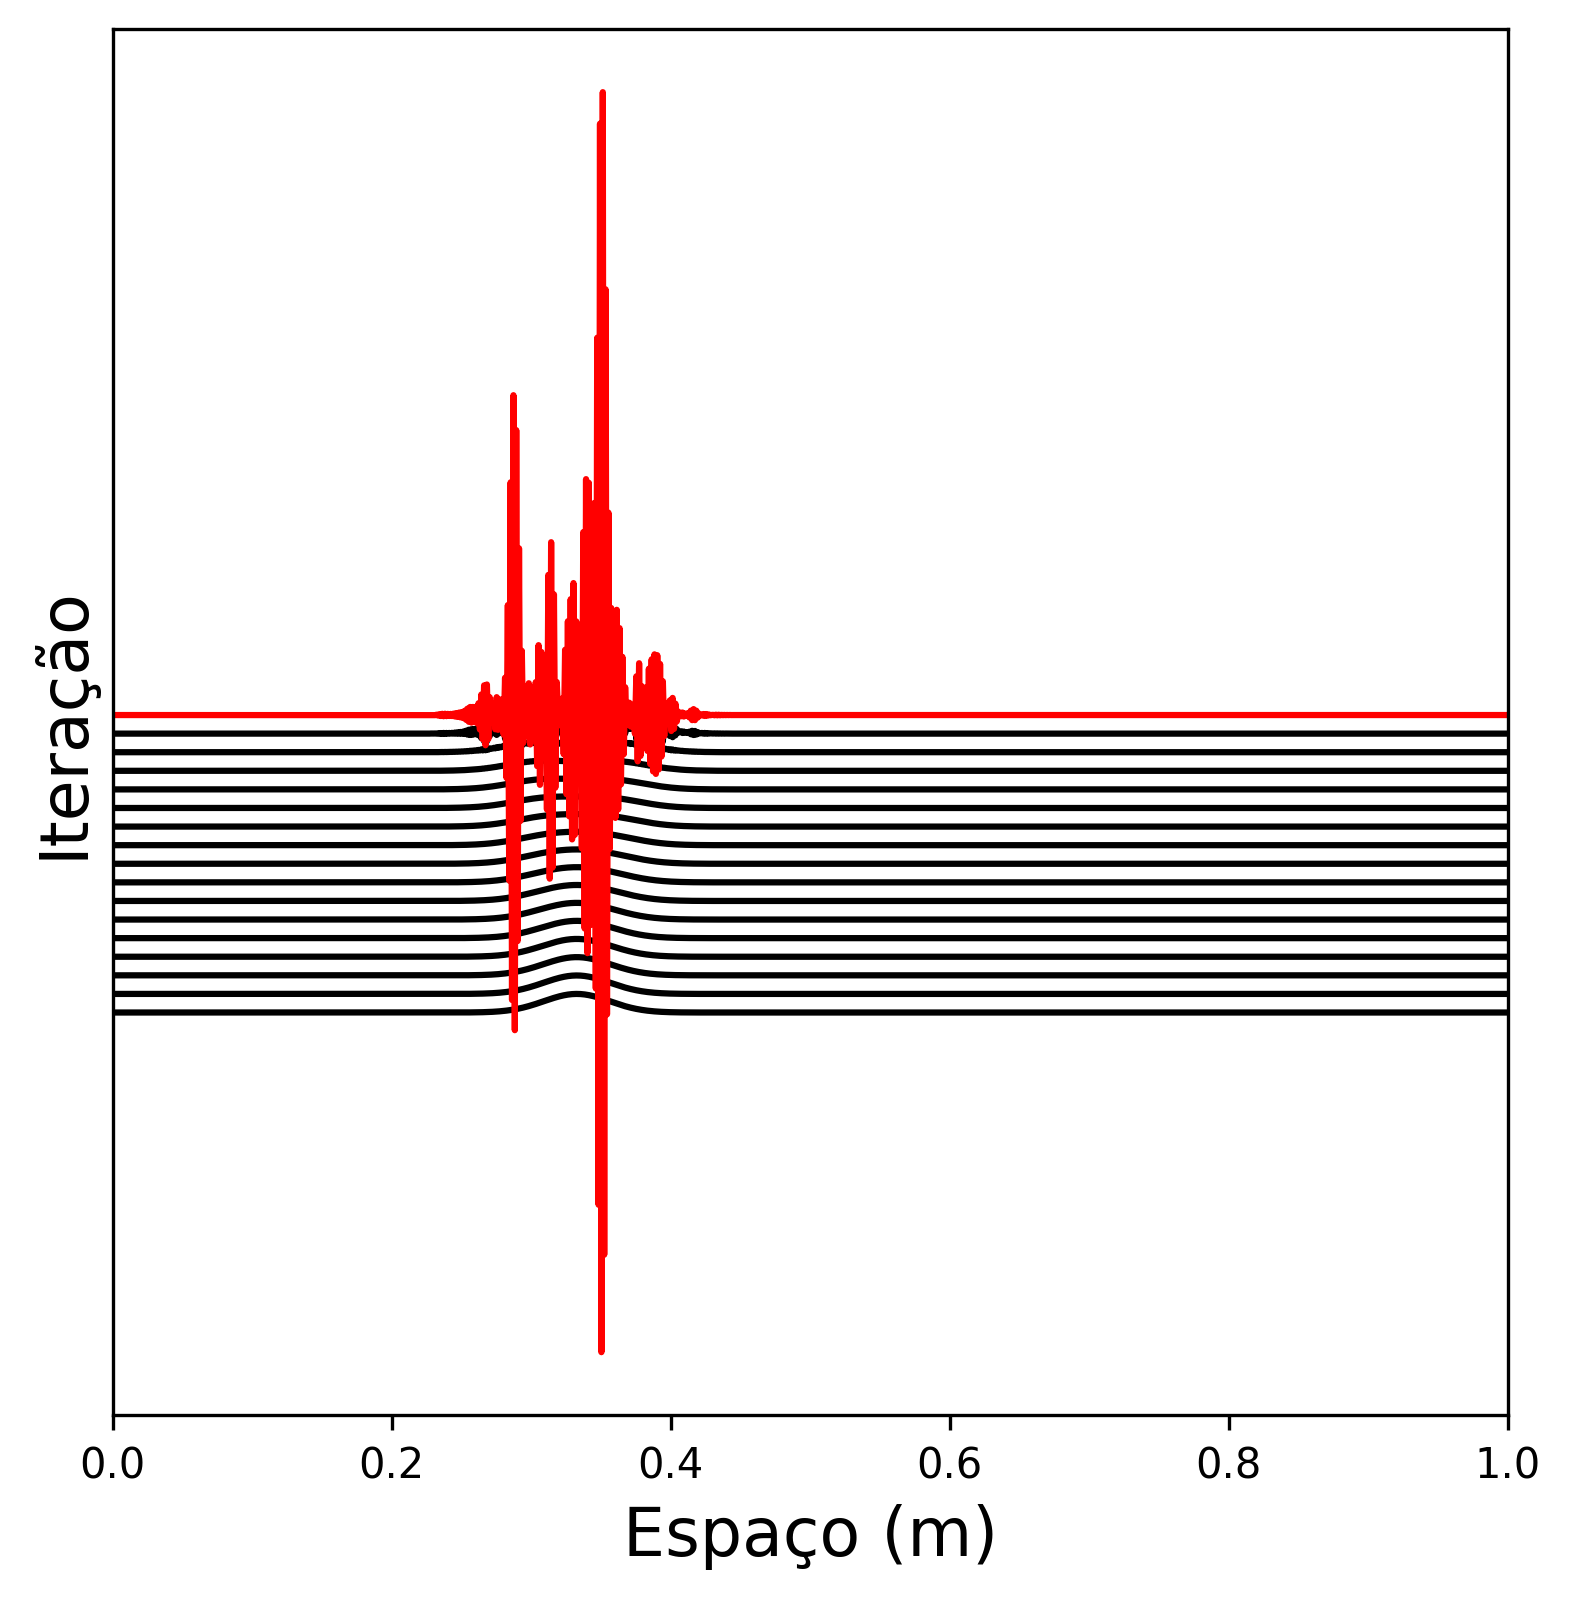
\includegraphics[width=0.5\linewidth]{graf-tarefa1-b}
    \label{fig:tarefa1-b}
\end{figure}


\subsection{Caso de \( r = 0.25 \) }

A implementação com valores de \( r < 1 \) apresentam certa estabilidade, como pode ser observado
na figura (\ref{fig:tarefa1-c1}), porém para tempos grandes surgem deformações no
pacote gaussiano. E além disso, para tempos pequenos apesar de simular bem, não é eficiente
computacionalmente, já que executa muito mais iterações que no caso de \( r = 1 \)\footnote{Nota-se, que assim como
        foi dito, o número de iterações aumenta.  Para \( r = 0.25 \), ou seja \( 1/4 \) do \( r \) anterior, o número de iterações quadriplica.}
. Isso porque, para
\( \Delta x \), \( c \) e \( r \) fixos, precisamos alterar o parâmetro de \( \Delta t \), o que aumenta
o número de iterações do nosso programa.

Para conseguir observar o surgimento das deformações foi necessário diminuir a precisão da grade
para \( 10^{-2} \), pois utilizando o \( \Delta x \) de ordem \( 10^{-3} \) não consegui observar as
instabilidades. Foi testado para diversos tempos e não exibiu em nenhum momento deformações como as
da (\ref{fig:tarefa1-c2}). Como podemos ver, a escolha de \( \Delta x\) impactou bastante o desempenho
dessa simulação.

\begin{figure}[h!] 
    \centering
    \caption{Simulação para \( r = 0,25 \) nas primeiras iterações.}
    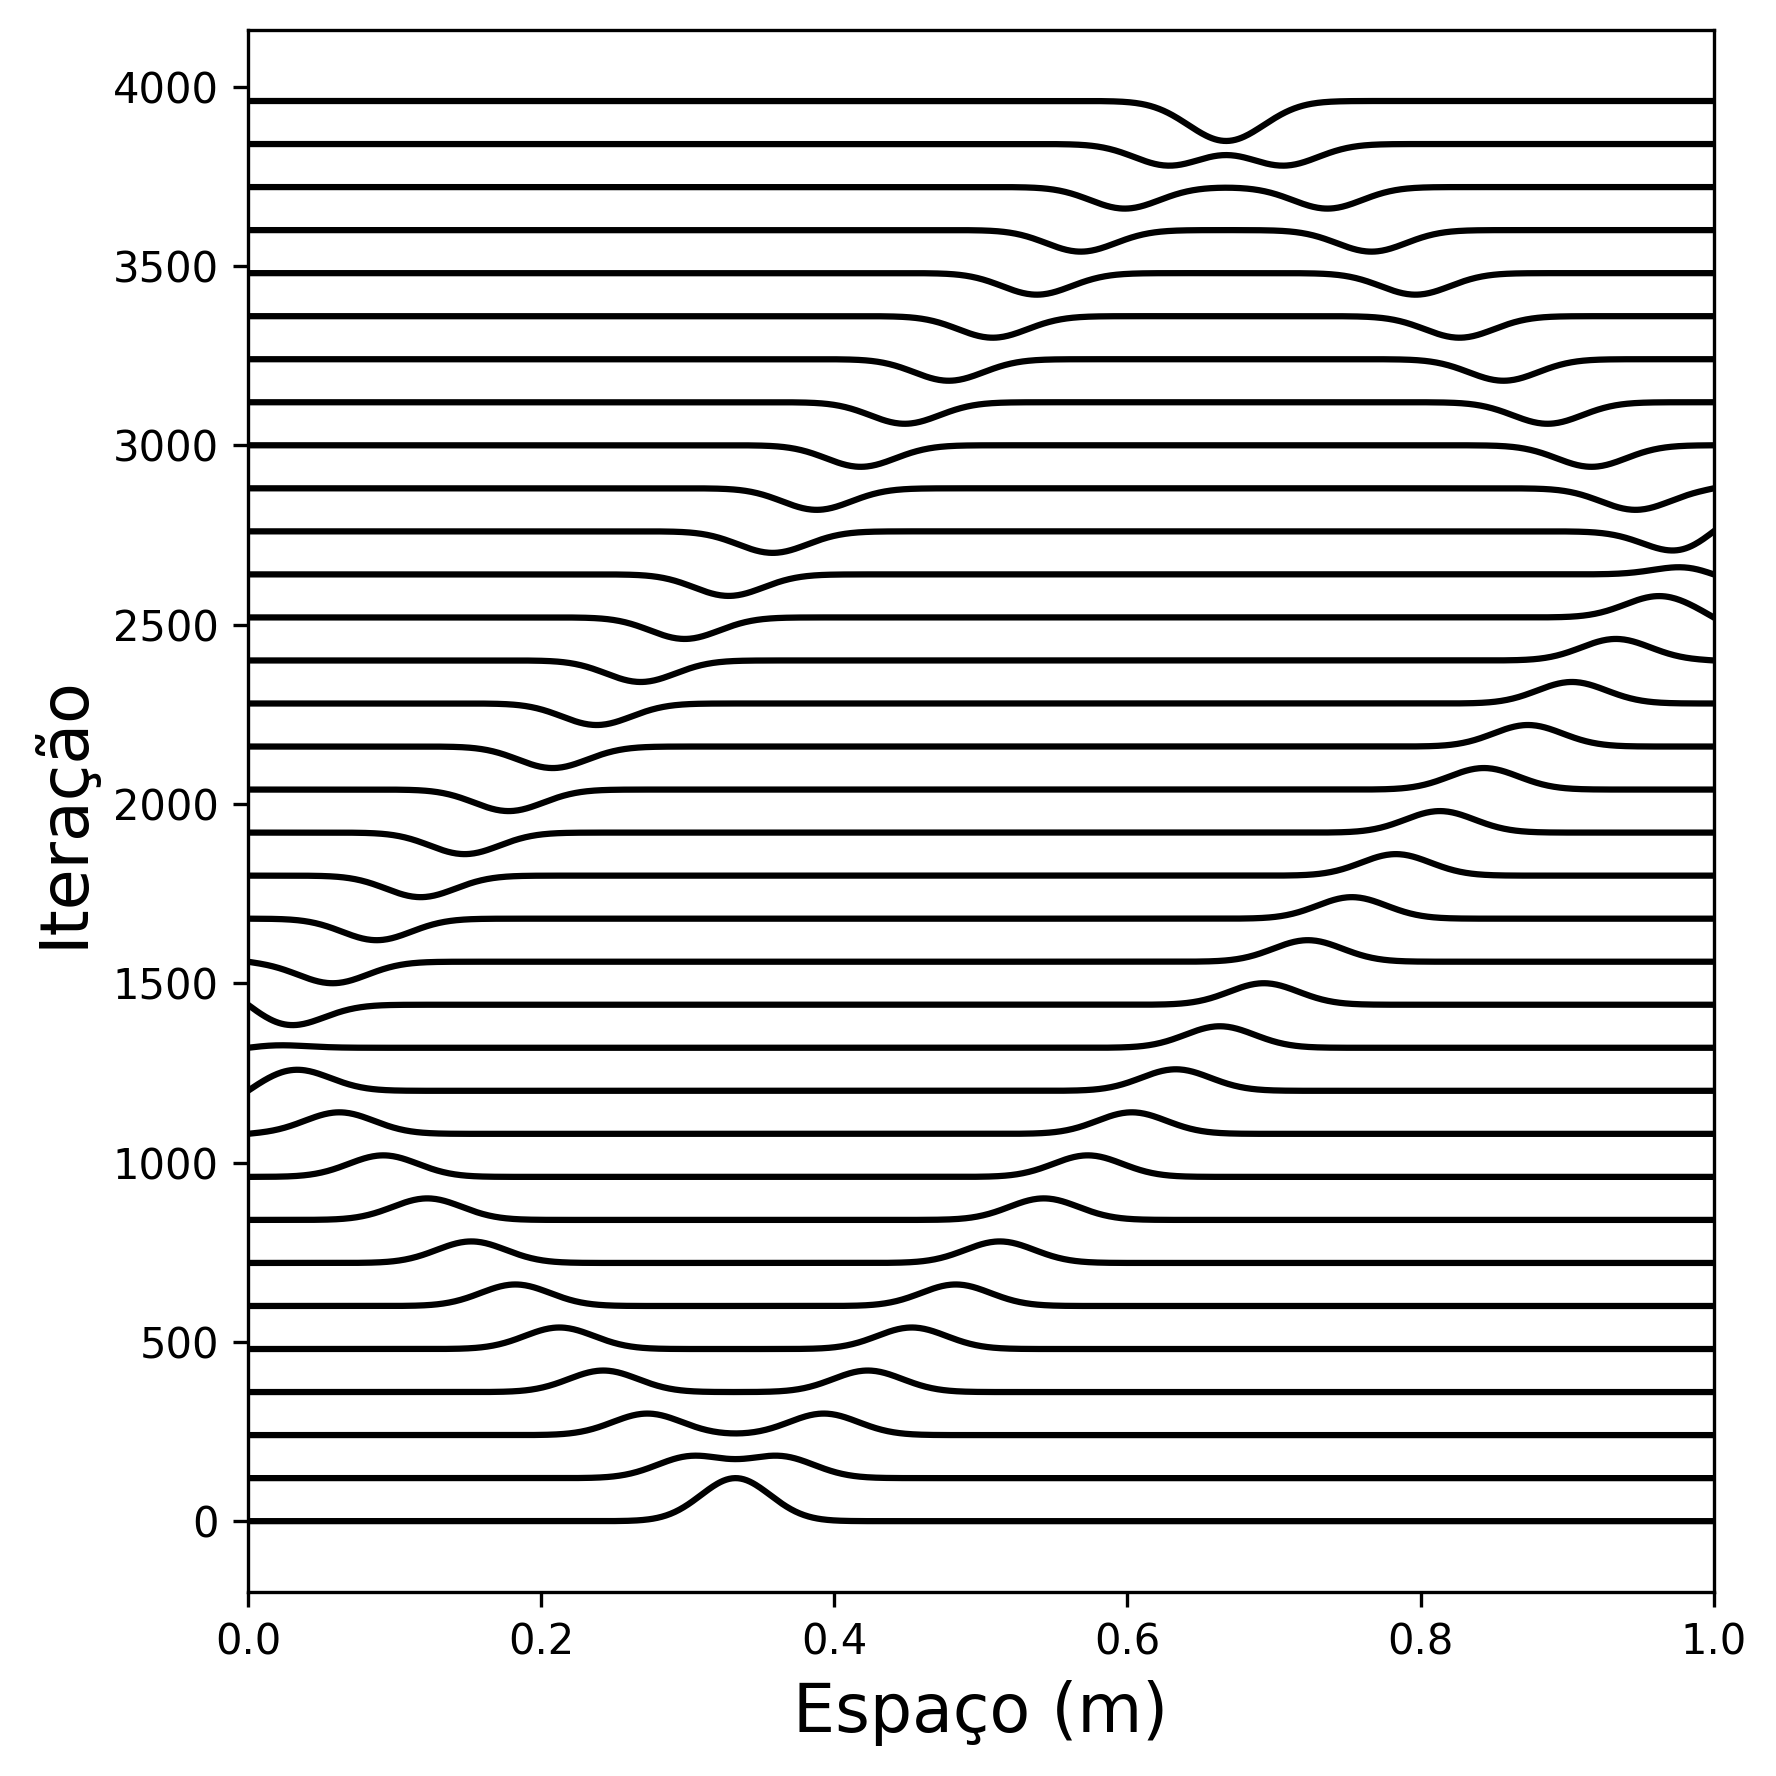
\includegraphics[width=0.5\linewidth]{graf-tarefa1-c1}
    \label{fig:tarefa1-c1}
\end{figure}



A figura (\ref{fig:tarefa1-c2}) foi construída a partir da simulação com \( r = 0.25 \) e \( t = 0,02
\) e com \( \Delta x = 10^{-2}\). No gráfico temos o comportamento da onda para um tempo grande, após muita iterações e podemos
ver claramente as deformações do pacote gaussiano.

\begin{figure}[h!] 
    \centering
    \caption{Comportamento da onda para um tempo grande.}
    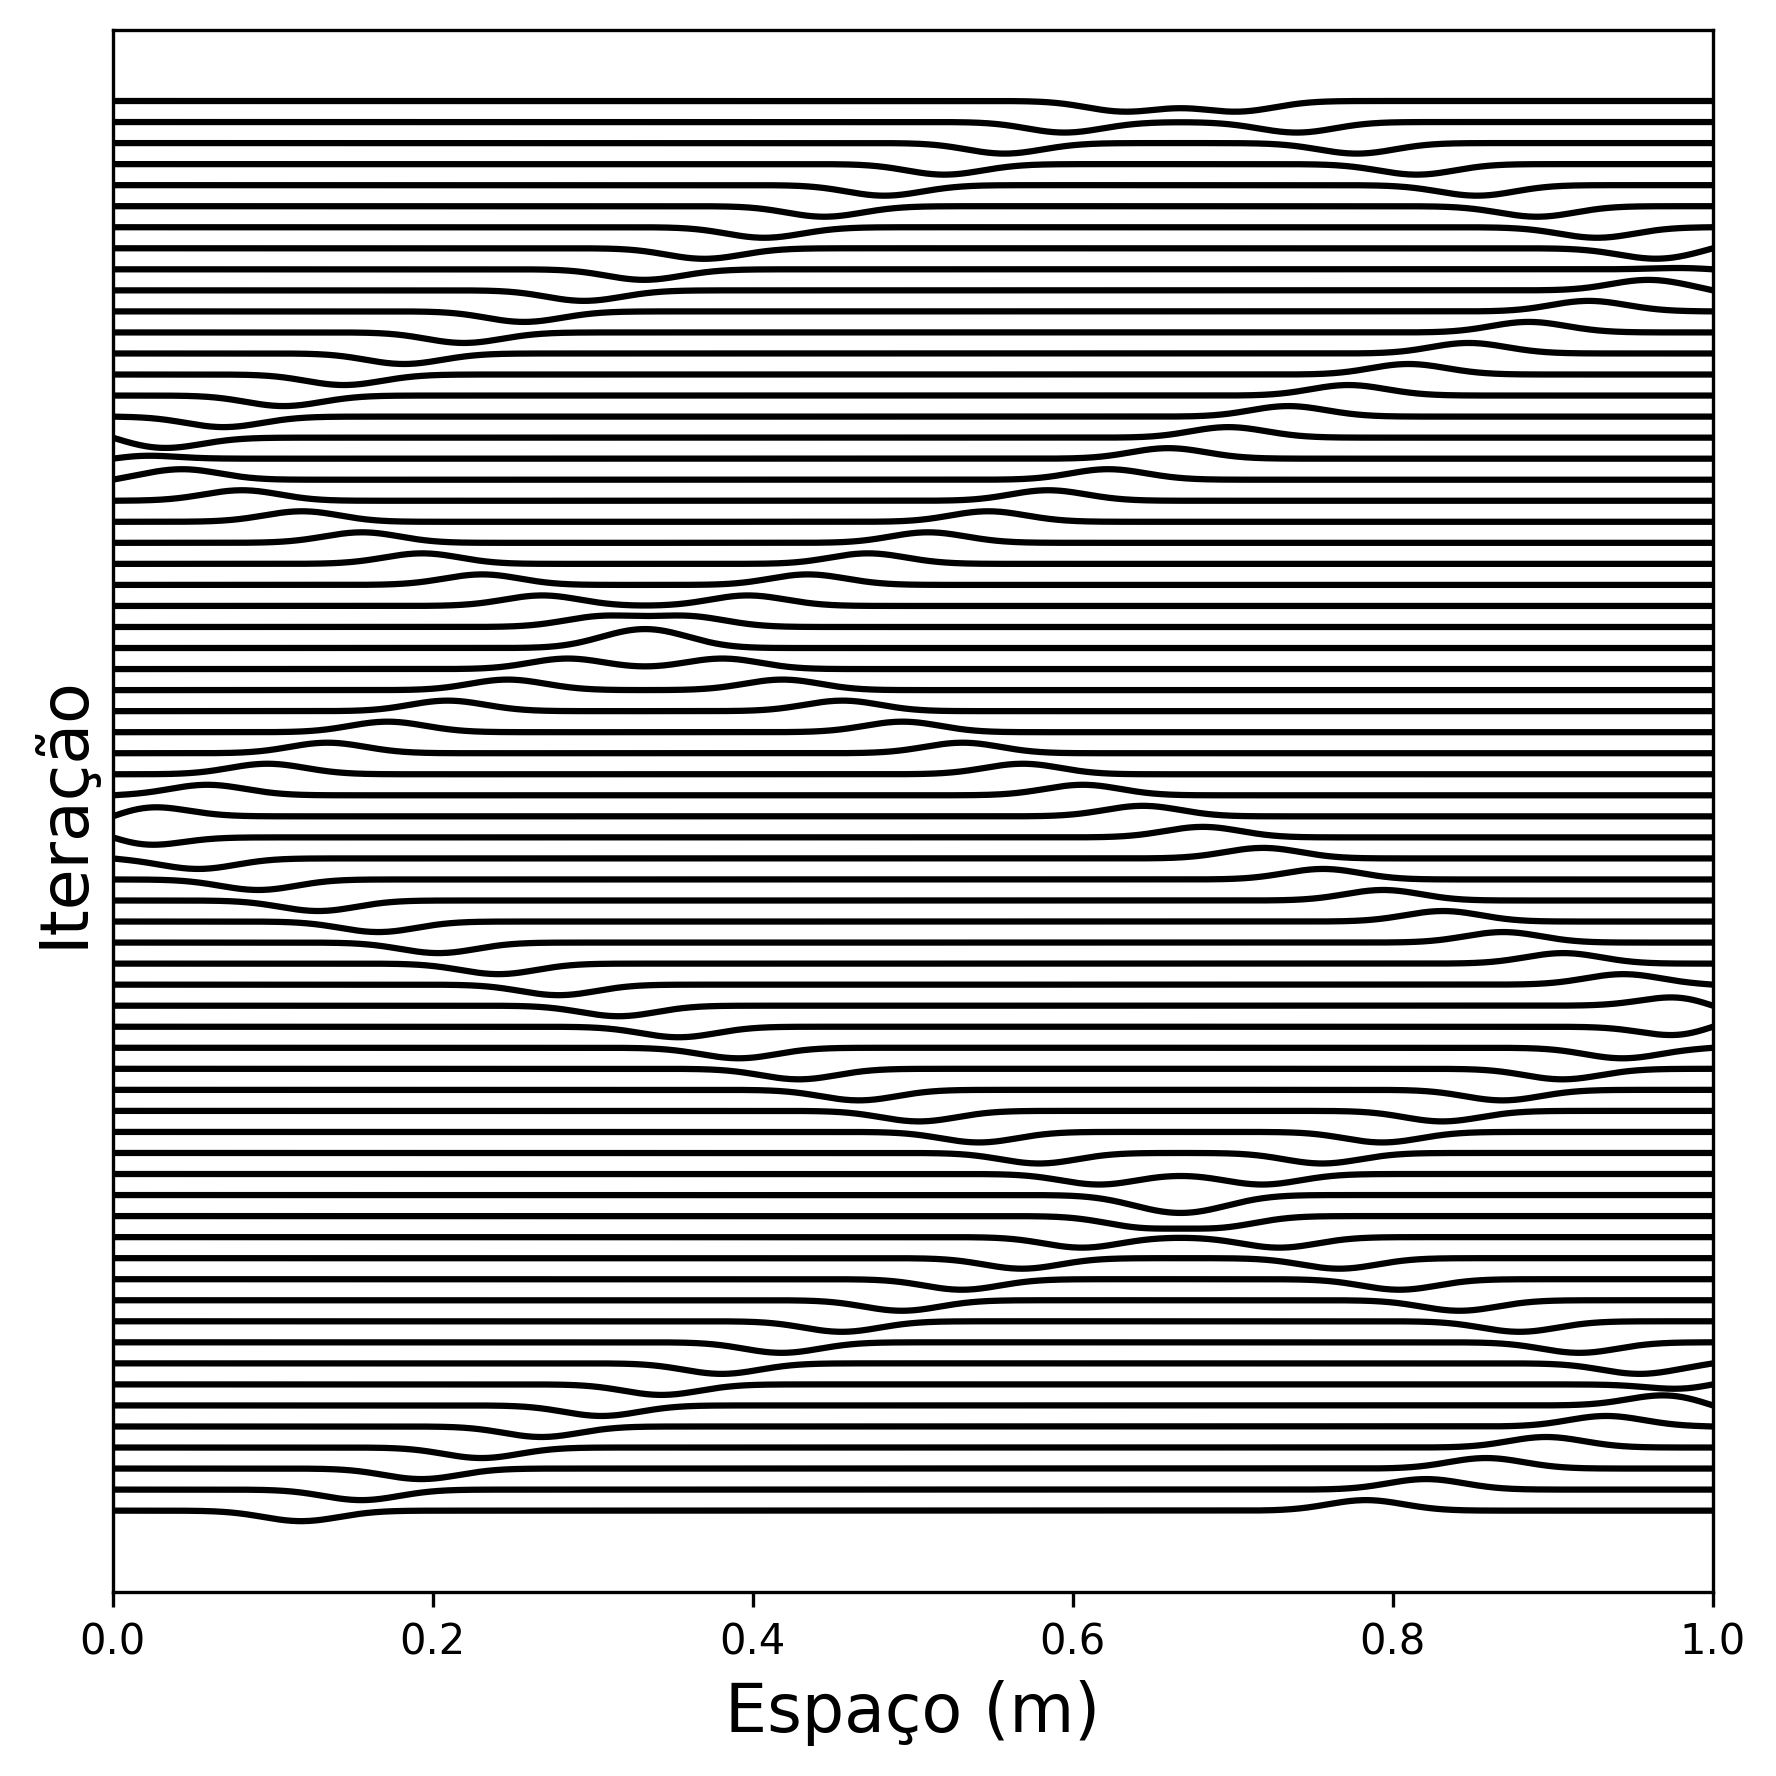
\includegraphics[width=0.50\linewidth]{graf-tarefa1-c2}
    \label{fig:tarefa1-c2}
\end{figure}


\section{Simulação de ondas na corda de violão}

Já o perfil inicial de pinça, na corda do violão, foi chamado de \verb|Y0_pinca(x, s)|, e pela
figura dada no projeto temos que o perfil inicial da onda deverá ser 

\begin{equation}
  \mathcal{Y}(x, 0) = \mathcal{Y}_0(x) = \begin{cases}
    x, x < L/4\\
    \frac{1}{3} \left( L - x \right), L/4 \leq x \leq L
  \end{cases}
  \label{eq:y_0_pinca}
\end{equation}


O código da implementação dessa simulação é diferente em relação ao primeiro apenas nas condições
iniciais. Portanto apenas compilarei no relatório esse trecho diferente dos programas:

\begin{minted}{fortran}[!]
      function Y0_pinca(x, s)
      implicit real*8(a-h, o-y)
      if(x .le. s/4) then
         Y0_pinca = x
      else
         Y0_pinca = (1.0e0/3.0e0)*(s - x)
      end if
      end
\end{minted}


\subsection{Caso de \( r = 1 \) }
Nesse caso o pacote não se deforma e como podemos ver, os pacotes menores sofrem reflexões
nas próximo das iterações em torno de $250$ e $780$, comportamento igual ao do primeiro caso observado
anteriormente. E assim como nele, também vai haver repetição da configuração inicial em um tempo
igual à \( t = 2L/c \), ou seja, ambos pacotes menores devem andar \( 2L \) antes de haver a
repetição da situação inicial. E por fim, as interferências também são como antes: construtivas.

\begin{figure}[h!] 
    \centering
    \centering
    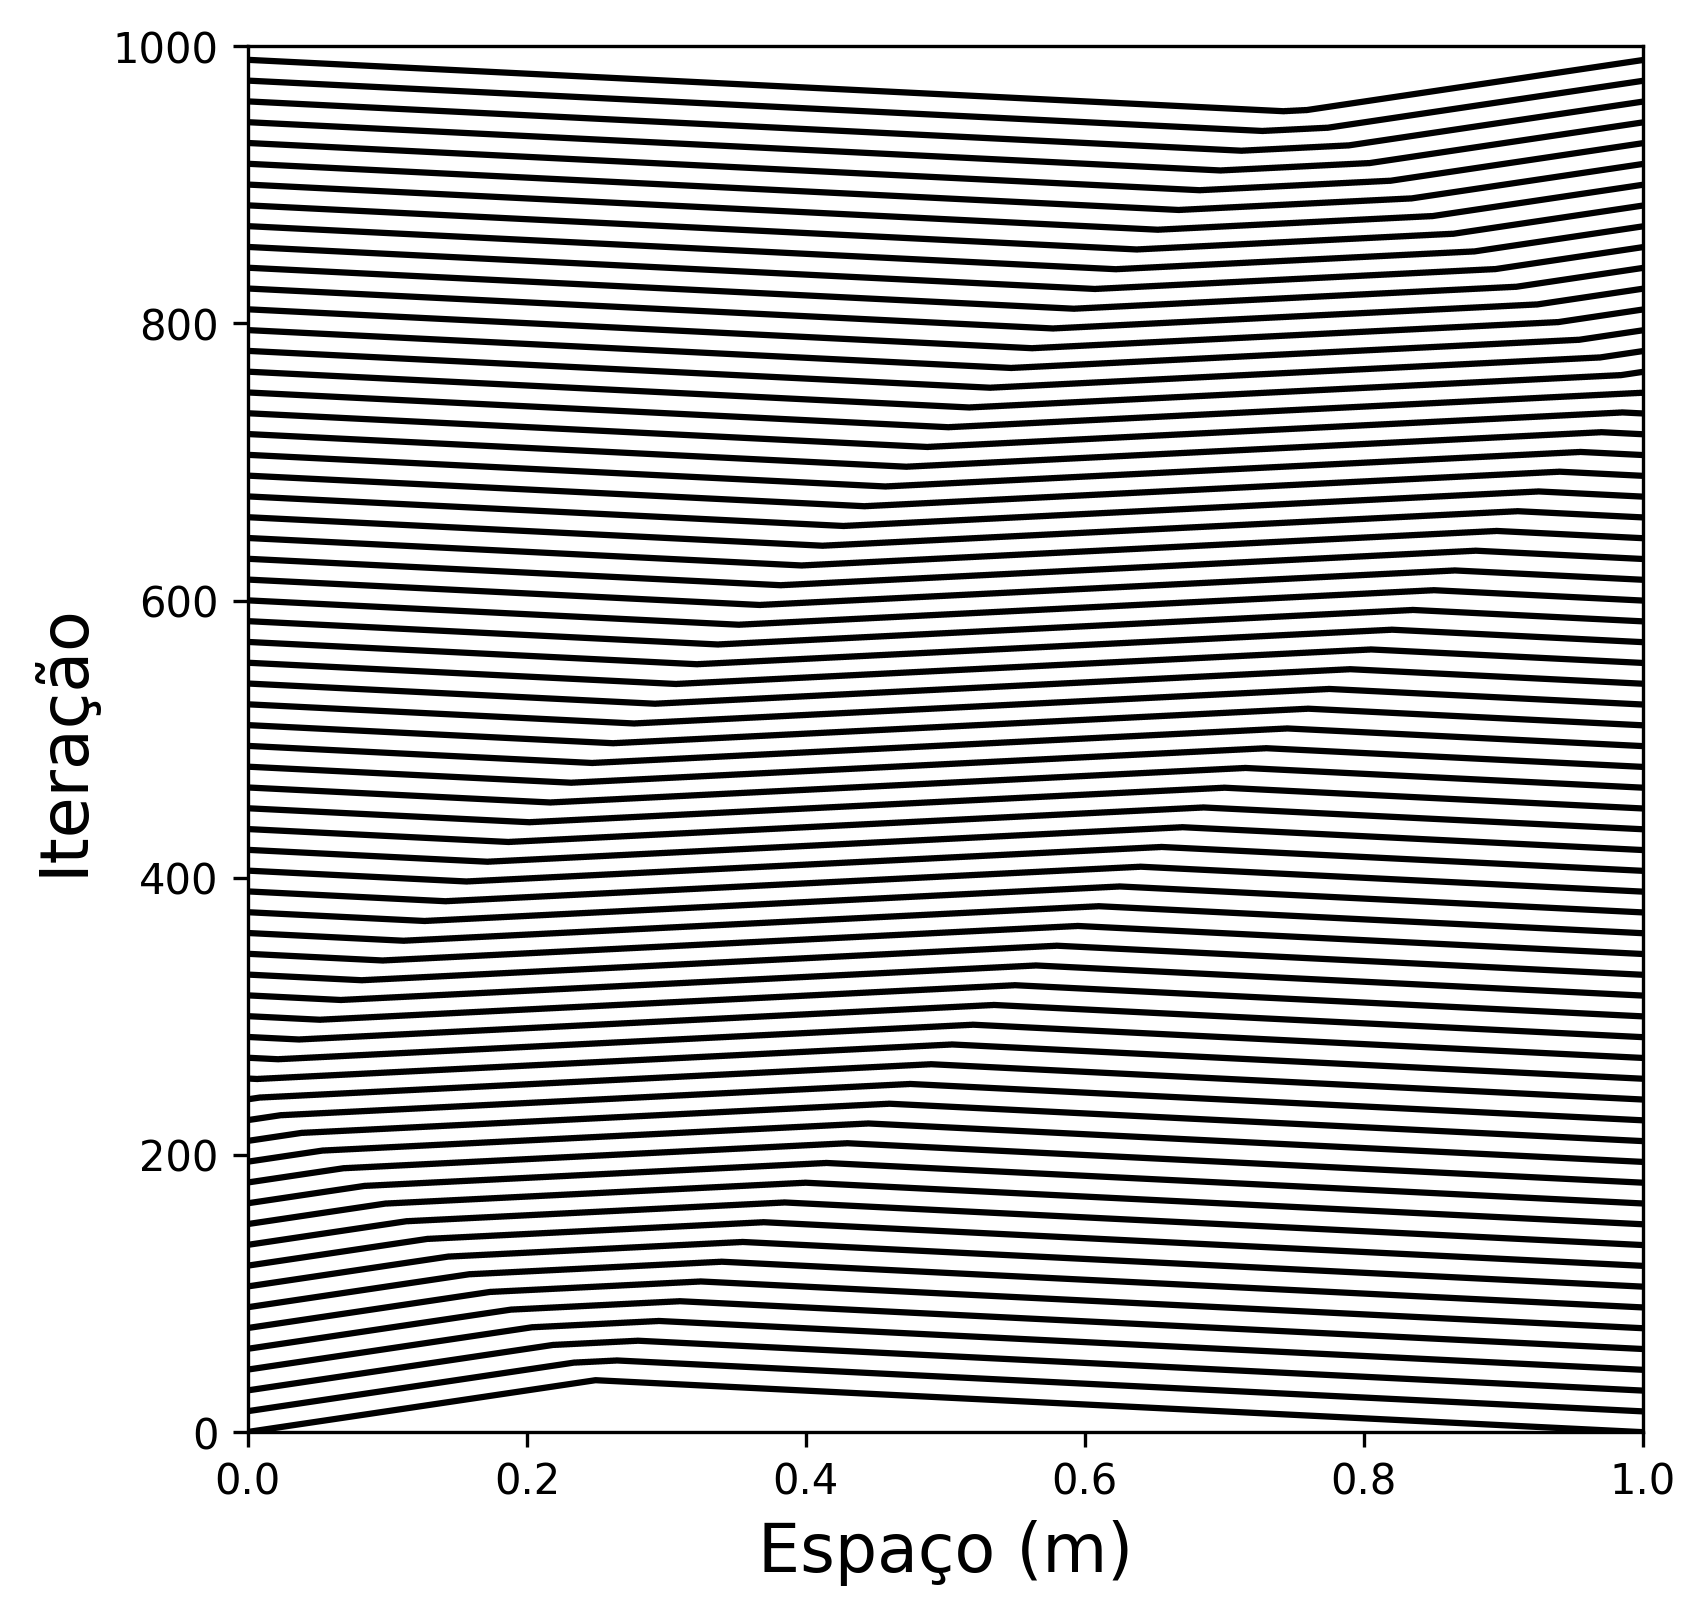
\includegraphics[width=0.5\linewidth]{graf-tarefa2-a}
    \caption{}
    \label{fig:subA}
\end{figure}


\subsection{Caso de \( r = 2 \) }

Esse caso é similar ao da tarefa anterior (\ref{sec:caso_r_2}). Nesse caso temos a especifidade da
divergencia acontecer muito mais rapido que no anterior. Suponho que isso esteja relacionado ao
perfil inicial da onda, já que nesse perfil temos muitos pontos diferentes de zero, ao contrário do
perfil dos pacotes gaussianos. Esses valores se acumulam mais rapidamente que na
(\ref{sec:caso_r_2}). Além disso a divergência parece acontecer somente no ponto \( x = L/3 \).

O motivo disso pode ser justamente as condições iniciais, já que na gaussiana boa parte dos valores
inciais da grade é nulo, e na condição de pinça (\ref{eq:y_0_pinca}) temos valores maiores que
contribuem para as próximas iterações que como vimos são ampliadas muitos rapidamente.

\begin{figure}[h!] 
    \centering
    \caption{Simulação das ondas divergindo para \( r = 2 \) em poucas iterações.}
    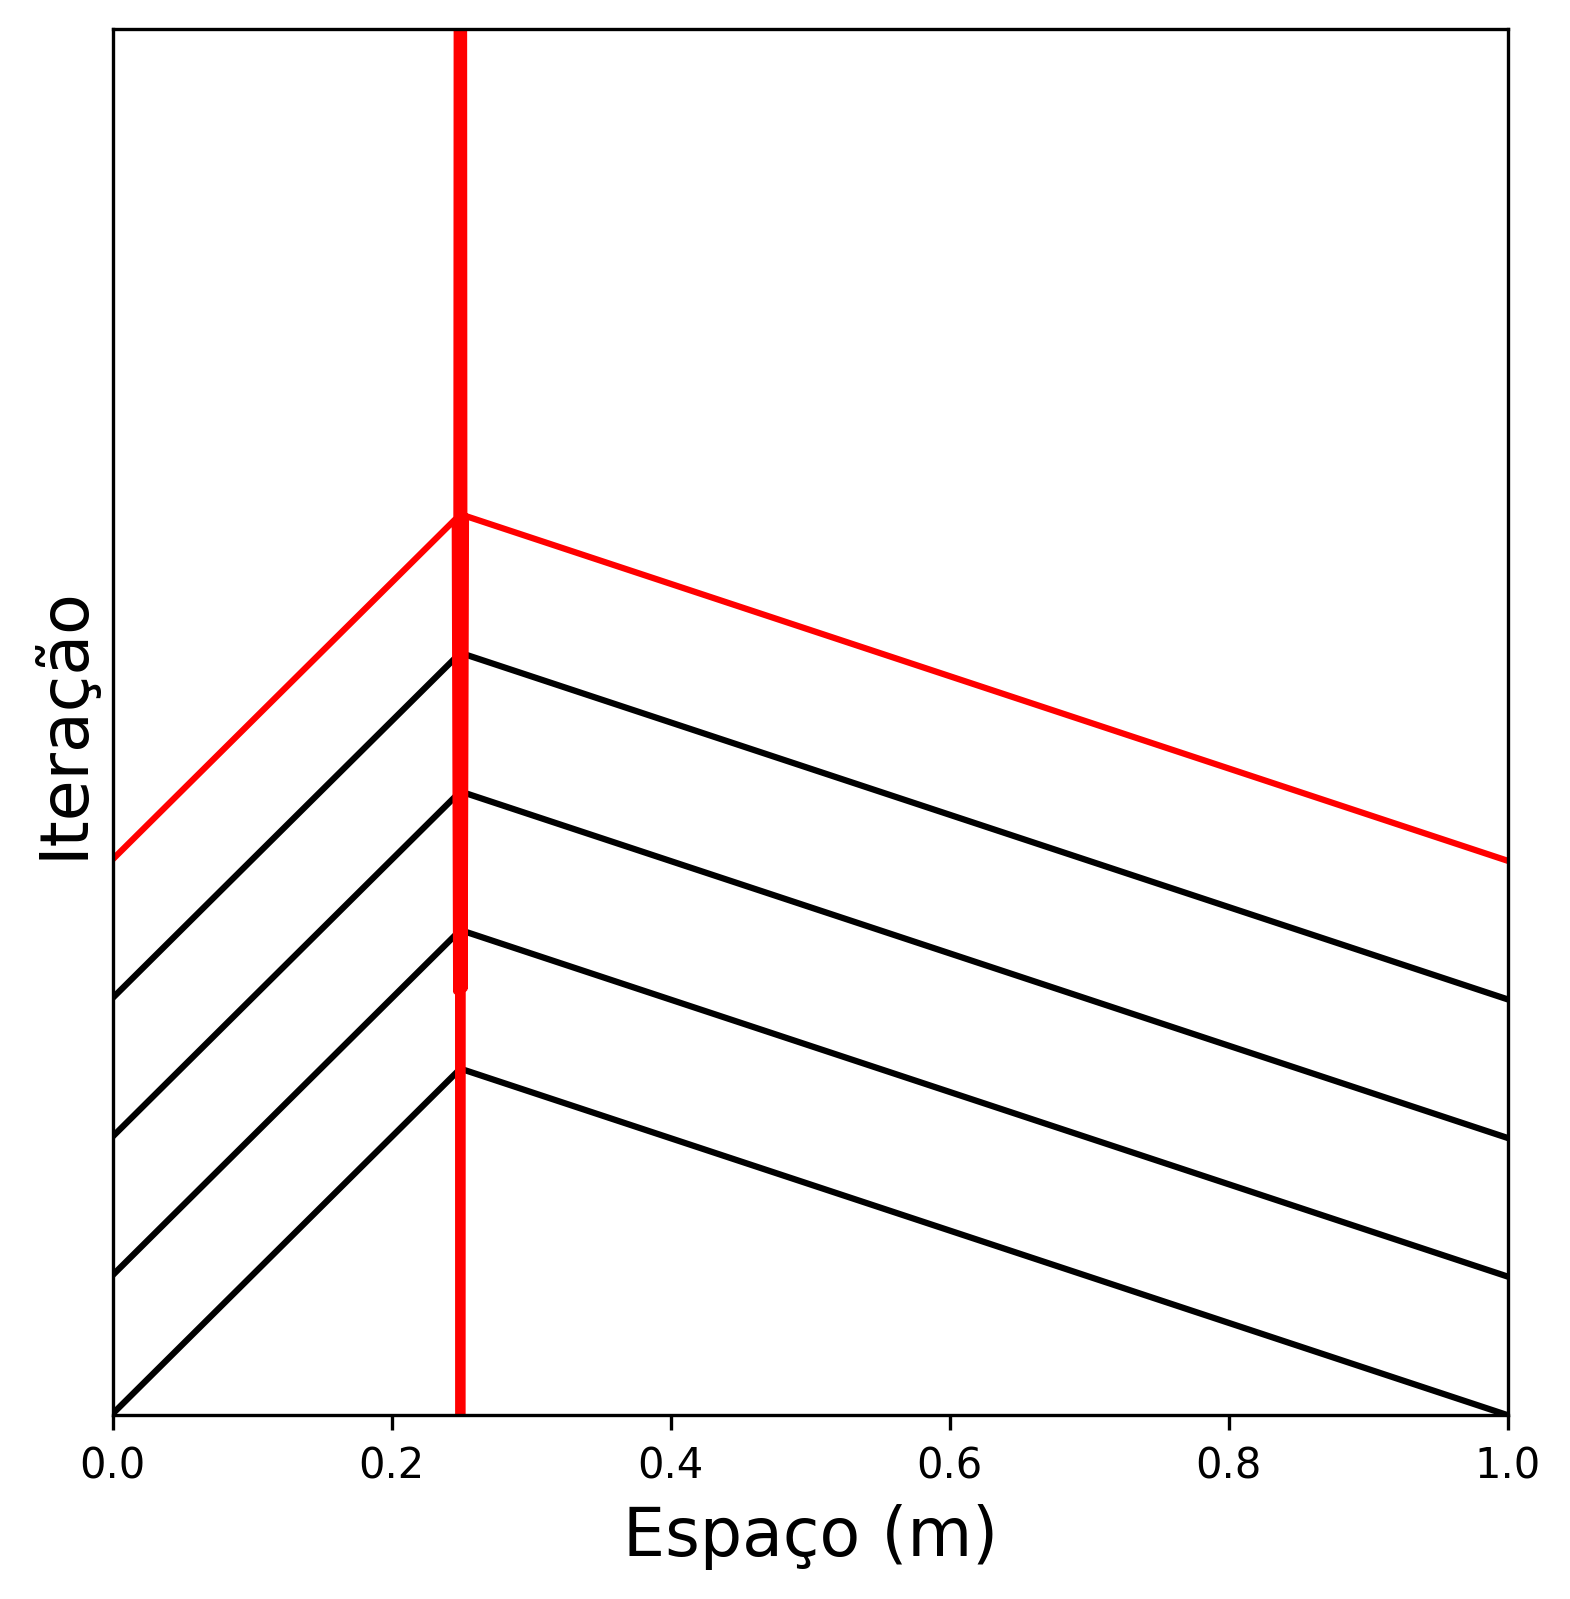
\includegraphics[width=0.5\linewidth]{graf-tarefa2-b}
    \label{fig:subB}
\end{figure}



\subsection{Caso de \( r = 0.25 \) }

\begin{figure}[h!] 
    \centering
    \caption{Simulação das ondas no violão para \( r = 0,25 \). }
    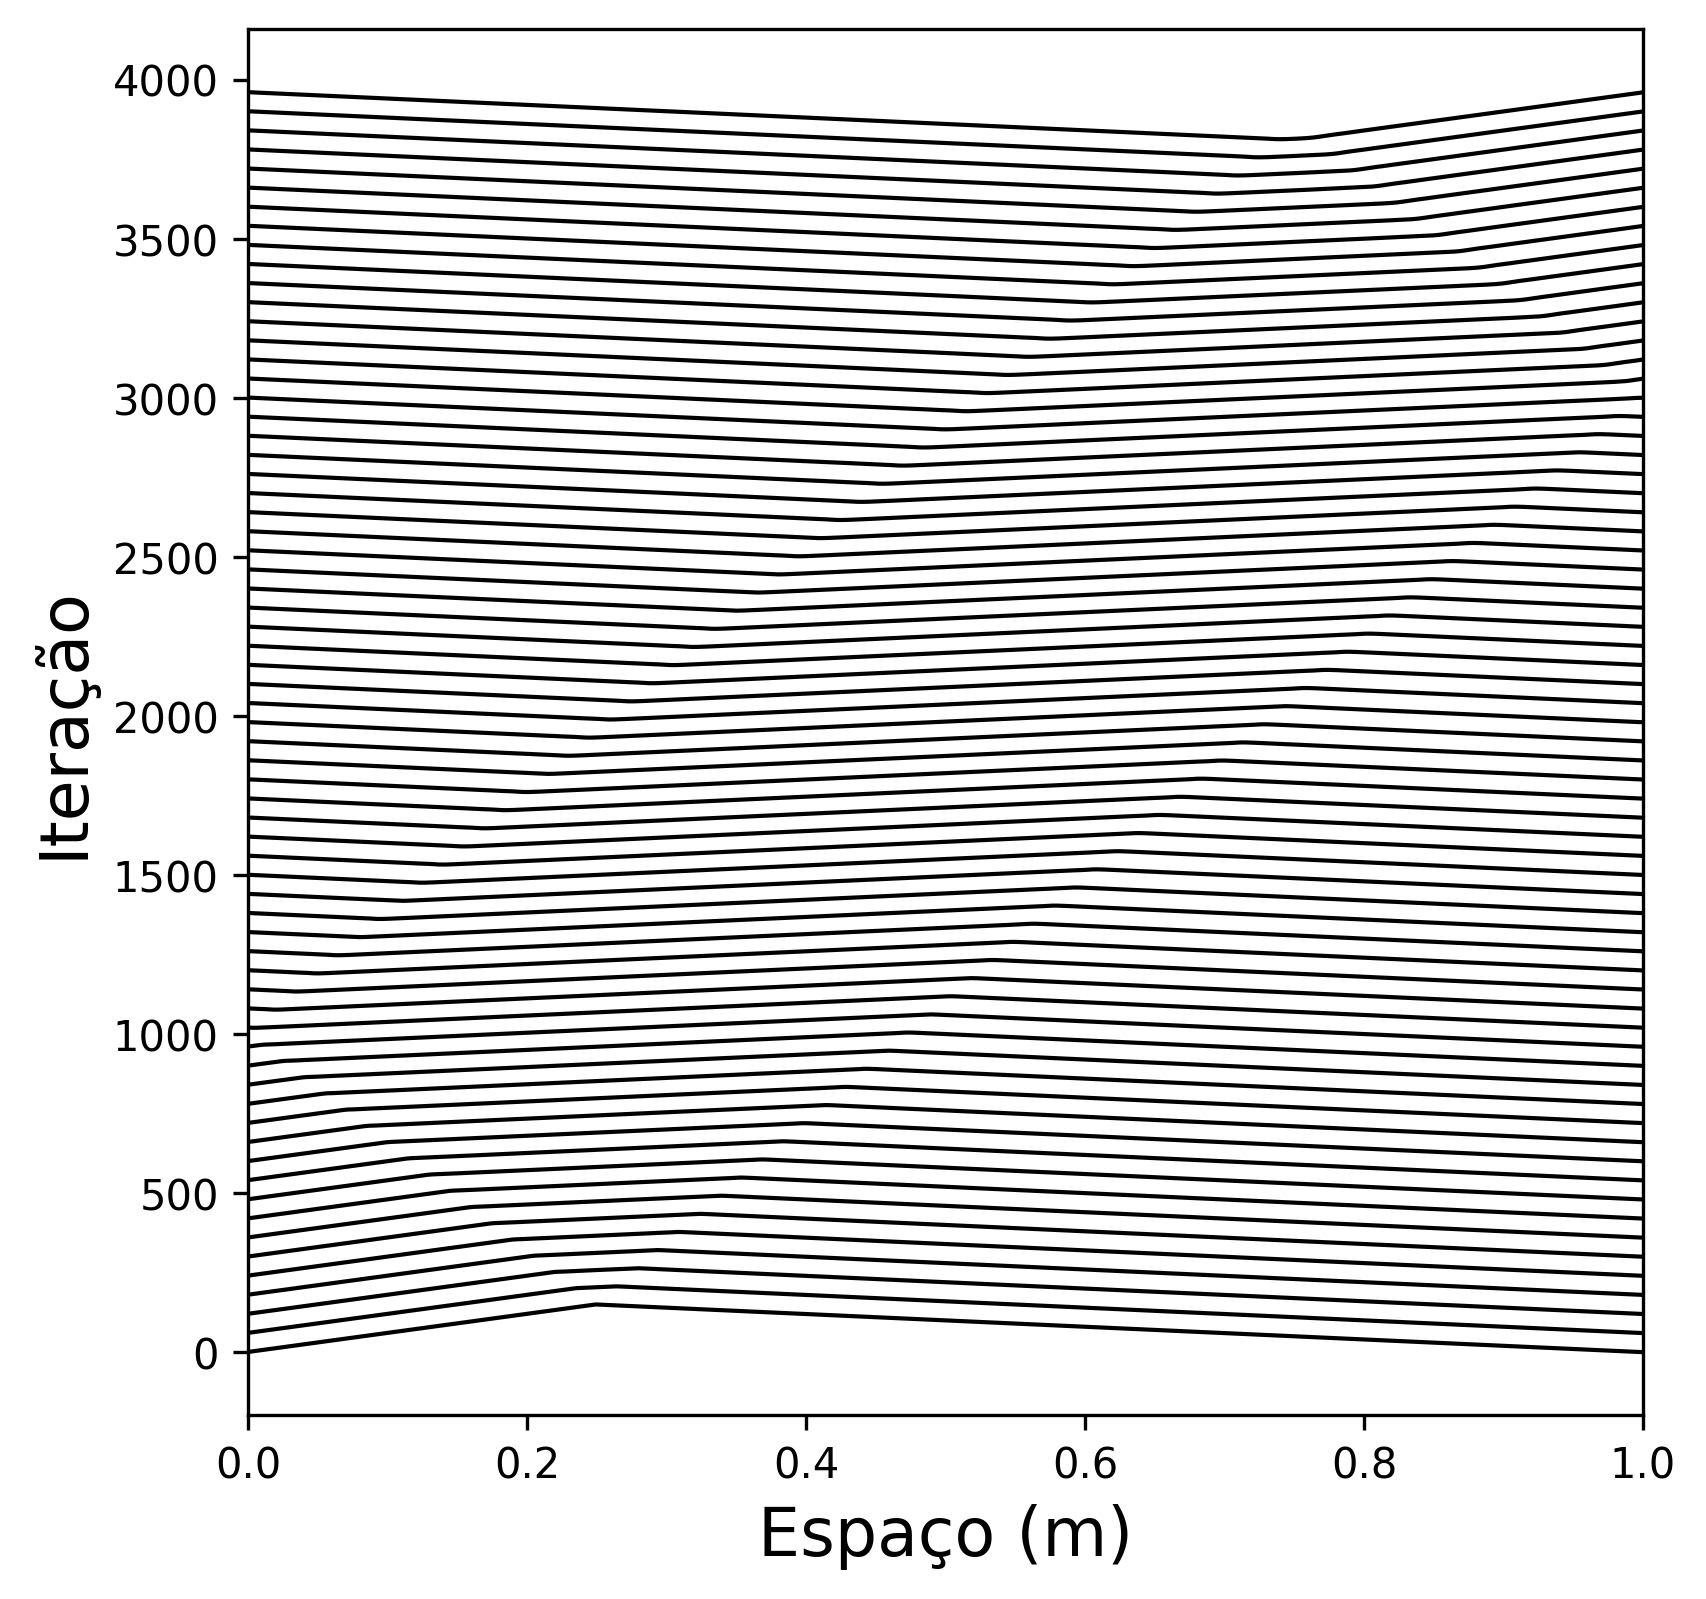
\includegraphics[width=0.5\linewidth]{graf-tarefa2-c1}
    \label{fig:tarefa2_c1}
\end{figure}

Assim como na tarefa anterior também foi simulado o sistema para \( \Delta x = 10^{-2} \) para tentar
observar as instabilidades. Para \( \Delta x = 10^{-3} \) não foi possível ver deformações para todos
tempos testados.
\begin{figure}[h!] 
    \centering
    \caption{Gráfico simplificado das deformações de ondas para condição inicial (\ref{eq:y_0_pinca}).}
    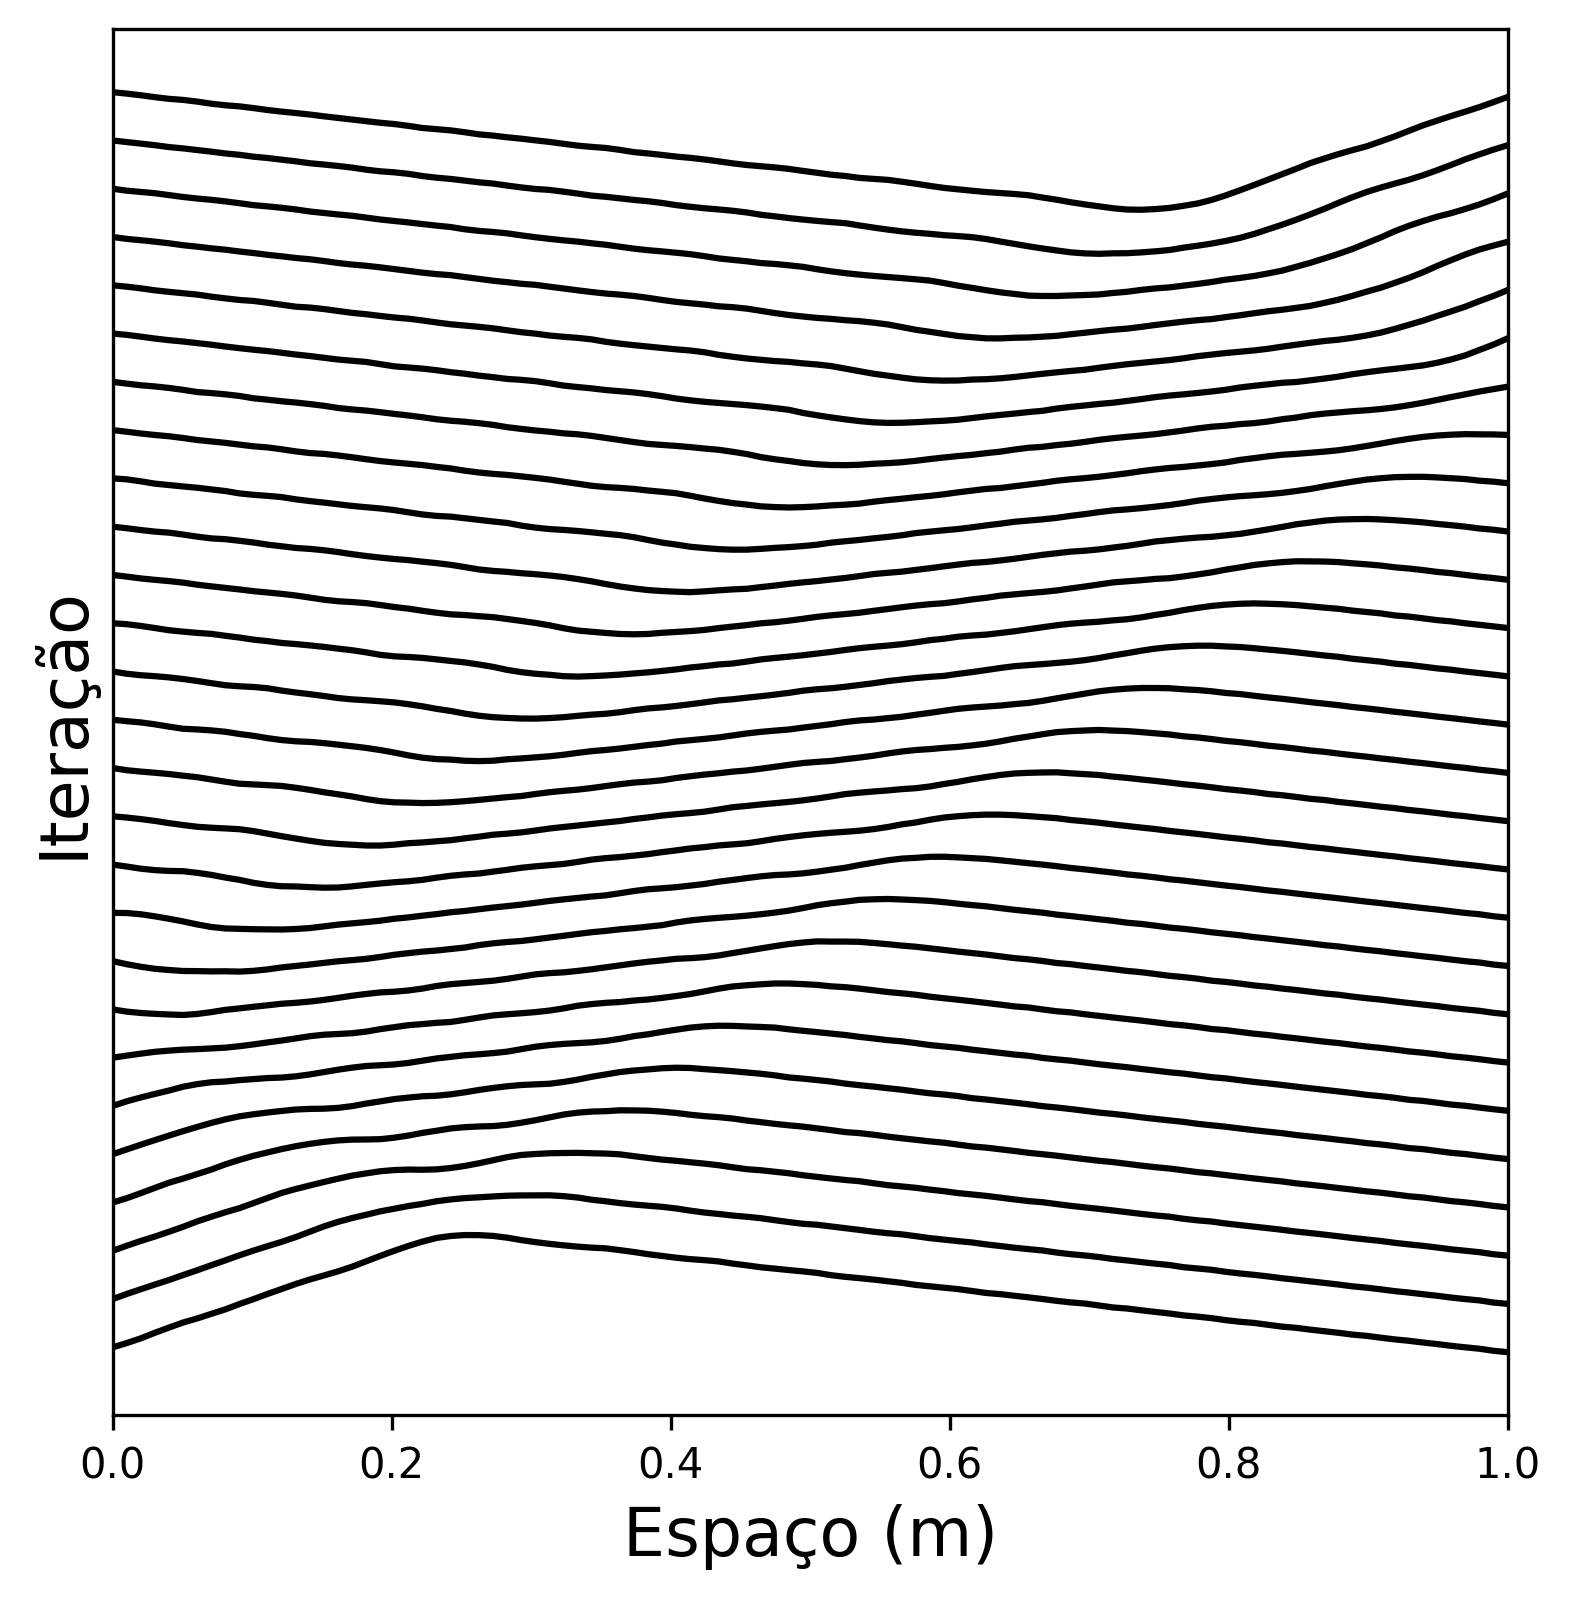
\includegraphics[width=0.5\linewidth]{graf-tarefa2-c22}
    \label{fig:tarefa2_c}
\end{figure}

Apesar de difícil de perceber, podemos notar as deformações na propagação, sobretudo nas regioes de
\( x \approx 0,3 \) e \( x \approx 0,7\) que são pontos de interferência.

\end{document}
%%% Local Variables:
%%% mode: latex
%%% TeX-master: "main.tex"
%%% End:
